%%%%%%%%%%%%%%%%%%%%%%%%%%%%%%%%%%%%%%%%%%%%%%%%%%%%%%%%%%%%%%%%%%%%%%%%%
\section{Experimental Evaluation}  %%%%%%%%%%%%%%%%%%%%%%%%%%%%%%%%%%%%%%
\label{cr:sec:experiments}

% Think of the difference between *predictive* and *explanatory*.
In this section, we investigate
\begin{enuminline}
\item the ability of the network choice model to accurately recover transitions in real-world scenarios, and
\item the potential of ChoiceRank to scale to very large networks.
\end{enuminline}

\subsection{Accuracy on Real-World Data}
\label{cr:sec:accuracy}

We evaluate the network choice model on three datasets that are representative of two distinct application domains.
%The first dataset contains clickstream data from the English Wikipedia, i.e., traces of users' navigation on a Web site.
%The second dataset consists of the records of all trips made using New York City's bicycle-sharing service during the year 2015, i.e., mobility traces in a large city.
Each dataset can be represented as a set of transition counts $\{ c_{ij} \}$ on a directed graph $G = (V,E)$.
We aggregate the transition counts into marginal traffic data $\{ (c^-_i, c^+_i) \mid i \in V \}$ and fit a network choice model by using ChoiceRank.
We set $\alpha = 2.0$ and $\beta = 1.0$ (these small values simply guarantee the convergence of the algorithm) and declare convergence when $\lVert \bm{\lambda}^{(t)} - \bm{\lambda}^{(t-1)} \rVert_1 / n < 10^{-8}$.
Given $\bm{\lambda}$, we estimate transition probabilities using $p_{ij} \propto \lambda_j$ as given by \eqref{cr:eq:singlelik}.
To the best of our knowledge, there is no other published method tackling the problem of estimating transition probabilities from marginal traffic data.
Therefore, we compare our method to three baselines based on simple heuristics.
\begin{description}[topsep=1ex,itemsep=0ex]
\item[Traffic] Transitions probabilities are proportional to the traffic of the target node: $q_{ij}^T \propto c_j^{-}$.
\item[PageRank] Transition probabilities are proportional to the PageRank score of the target node: $q_{ij}^P \propto \text{PR}_j$.
\item[Uniform] Any transition is equiprobable: $q_{ij}^U \propto 1$.
\end{description}
The four estimates are compared against ground-truth transition probabilities derived from the edge traffic data: $p_{ij}^\star \propto c_{ij}$.
We emphasize that although per-edge transition counts $\{c_{ij}\}$ are needed to \emph{evaluate} the accuracy of the network choice model (and the baselines), these counts are not necessary for \emph{learning} the model---per-node marginal counts are sufficient.

Given a node $i$, we measure the accuracy of a distribution $\bm{q}_i$ over outgoing transitions using two error metrics, the KL-divergence and the (normalized) rank displacement:
\begin{align*}
D_{\text{KL}}(\bm{p}_i^\star, \bm{q}_i) &= \sum_{j \in N^+_i} p^\star_{ij} \log \frac{p^\star_{ij}}{q_{ij}}, \\
D_{\text{FR}}(\bm{p}_i^\star, \bm{q}_i) &= \frac{1}{\vert N^+_i \vert^2} \sum_{j \in N^+_i} \vert \sigma^\star_i(j) - \hat{\sigma}_i(j) \vert,
\end{align*}
where $\sigma^\star_i$ (respectively $\hat{\sigma}_i$) is the ranking of elements in $N^+_i$ by decreasing order of $p^\star_{ij}$ (respectively $q_{ij}$).
We report the distribution of errors ``over choices'', i.e., the error at each node $i$ is weighted by the number of outgoing transitions $c^+_i$.


\subsubsection{Clickstream Data}

\paragraph{Wikipedia}
The Wikimedia Foundation has a long history of publicly sharing aggregate, page-level web traffic data\footnote{See: \url{https://stats.wikimedia.org/}.}.
Recently, it also released clickstream data from the English version of Wikipedia \citep{wulczyn2016wikipedia}, providing us with essential ground-truth transition-level data.
We consider a dataset that contains information, extracted from the server logs, about the traffic each page of the English Wikipedia received during the month of March 2016.
Each page's incoming traffic is grouped by HTTP referrer, i.e., by the page visited prior to the request.
We ignore the traffic generated by external Web sites such as search engines and keep only the internal traffic (\num{18}\% of the total traffic in the dataset).
In summary, we obtain counts of transitions on the hyperlink graph of English Wikipedia articles.
The graph contains $n = \num{2316032}$ nodes and $m = \num{13181698}$ edges, and we consider slightly over \num{1.2} billion transitions over the edges.
On this dataset, ChoiceRank converges after \num{795} iterations.

\paragraph{Kosarak}
We also consider a second clickstream dataset from a Hungarian online news portal\footnote{The data is publicly available at \url{http://fimi.ua.ac.be/data/}.}.
The data consists of $\num{7029013}$ transitions on a graph containing $n = 41001$ nodes and $m = \num{974560}$ edges.
ChoiceRank converges after \num{625} iterations.

\begin{figure}
  \centering
  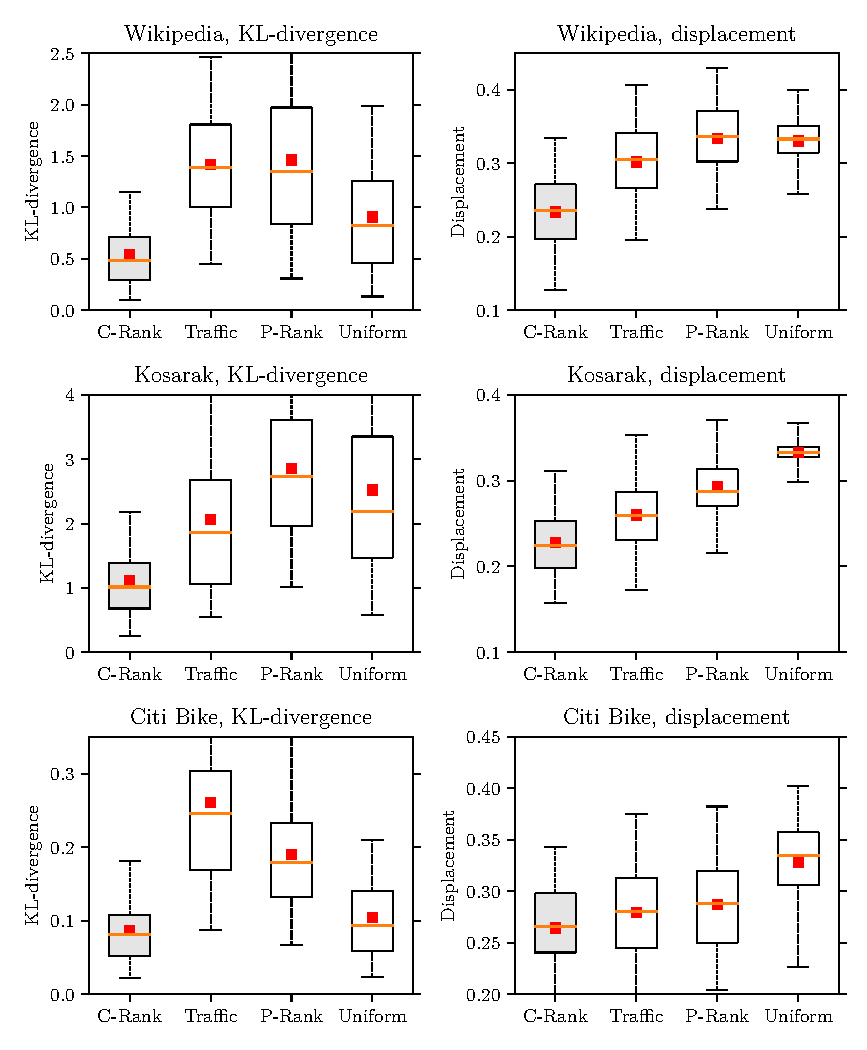
\includegraphics{cr-perf-combined}
  \caption{
Error distributions of the network choice model and three baselines for the Wikipedia (WP) and Citi Bike (CB) datasets.
The boxes show the interquartile range, the whiskers show the $5^{\text{th}}$ and $95^{\text{th}}$ percentiles, the red horizontal bars show the median and the red squares show the mean.
}
  \label{cr:fig:perf-combined}
\end{figure}

\begin{figure}[t]
  \centering
  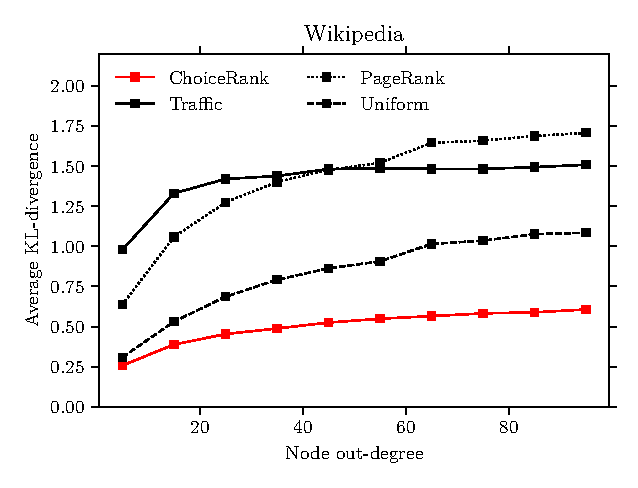
\includegraphics[width=0.6\linewidth]{cr-perf-wikipedia}
  \caption{
Average KL-divergence as a function of the number of possible transitions for the Wikipedia dataset.
ChoiceRank performs comparatively better in the case where a node's out-degree is large.
}
  \label{cr:fig:perf-wikipedia}
\end{figure}

The four leftmost plots of Figure~\ref{cr:fig:perf-combined} show the error distributions.
ChoiceRank significantly improves on the baselines, both in terms of KL-divergence and rank displacement.
These results give compelling evidence that transitions do not occur proportionally with the target's page traffic: in terms of KL-divergence, ChoiceRank improves on Traffic by a factor $3\times$ and $2\times$, respectively.
PageRank scores, while reflecting some notion of importance of a page, are not designed to estimate transitions, and understandably the corresponding baseline performs poorly.
Uniform (perhaps the simplest of our baselines) is (by design) unable to distinguish among transitions, resulting in a large displacement error.
We believe that its comparatively better performance in terms of KL-divergence (for Wikipedia) is mostly an artifact of the metric, which encourages ``prudent'' estimates.
Finally, in Figure~\ref{cr:fig:perf-wikipedia} we observe that ChoiceRank seems to perform comparatively better as the number of possible transition increases.


\subsubsection{NYC Bicycle-Sharing Data}

Next, we consider trip data from Citi Bike, New York City's bicycle-sharing system\footnote{The data is available at \url{https://www.citibikenyc.com/system-data}.}.
%Markov models have been used with success in the context of mobility prediction \citep{ashbrook2003using, kafsi2015traveling}. TODO
For each ride on the system made during the year 2015, we extract the pick-up and drop-off stations and the duration of the ride.
Because we want to focus on direct trips, we exclude rides that last more than one hour.
We also exclude source-destinations pairs which have less than 1 ride per day on average (a majority of source-destination pairs appears at least once in the dataset).
The resulting data consists of \num{3.4} million rides on a graph containing $n = \num{497}$ nodes and $m = \num{5209}$ edges.
ChoiceRank converges after $\num{7508}$ iterations.
We compute the error distribution in the same way as for the clickstream datasets.

The two rightmost plots of Figure~\ref{cr:fig:perf-combined} display the results.
The observations made on the clickstream datasets carry over to this mobility dataset, albeit to a lesser degree.
A significant difference between clicking a link and taking a bicycle trip is that in the latter case, there is a non-uniform ``cost'' of a transition due to the distance between source and target.
In future work, one might consider incorporating edge weights and using the weighted network choice model presented in Appendix~\ref{cr:app:extensions}.


\subsection{Scaling to Large Networks}

To demonstrate ChoiceRank's scalability, we develop a simple implementation in the Rust programming language, based on the ideas of COST \citep{mcsherry2015scalability}.
Our code is publicly available online\footnote{See: \url{http://lucas.maystre.ch/choicerank}.}.
The implementation repeatedly streams edges from disk and keeps four floating-point values per node in memory:
the counts $c^-_i$ and $c^+_i$, the sum of messages $z_i$, and either $\gamma_i$ or $\lambda_i$ (depending on the stage in the iteration).
As edges can be processed in any order, it can be beneficial to reorder the edges in a way that accelerates the computation.
For this reason, our implementation preprocesses the list of edges and reorders them in Hilbert curve order\footnote{A Hilbert space-filling curve visits all the entries of the adjacency matrix of the graph, in a way that preserves locality of both source and destination of the edges.}.
This results in better cache locality and yields a significant speedup.

We test our implementation on a hyperlink graph extracted from the 2012 Common Crawl web corpus\footnote{
The data is available at \url{http://webdatacommons.org/hyperlinkgraph/}.} that contains over \num{3.5} billion nodes and \num{128} billion edges \citep{meusel2014graph}.
The edge list alone requires about $1$ TB of uncompressed storage.
There is no publicly available information on the traffic at each page, therefore we generate a value $c_i$ for every node $i$ randomly and uniformly between \num{100} and \num{500}, and set both $c^-_i$ and $c^+_i$ to $c_i$.
As such, this experiment does not attempt to measure the validity of the model (unlike the experiments of Section~\ref{cr:sec:accuracy}).
Instead, it focuses on testing the algorithm's potential to scale to to very large networks.

\paragraph{Results}
We run \num{20} iterations of ChoiceRank on a dual Intel Xeon E5-2680 v3 machine, with \num{256} GB of RAM and \num{6} HDDs configured in RAID 0.
We arbitrarily set $\alpha = 2.0$ and $\beta = 1.0$ (but this choice has no impact on the results).
Only about \num{65} GB of memory is used, all to store the nodes' state ($4 \times 4$ bytes per node).
The algorithm takes a little less than \num{39} minutes per iteration on average.
Collectively, these results validate the feasibility of model inference for very large datasets.

It is worth noting that despite tackling different problems, the ChoiceRank algorithm exhibits interesting similarities with a message-passing implementation of PageRank commonly used in scalable graph-parallel systems such as Pregel \citep{malewicz2010pregel} and Spark \citep{gonzalez2014graphx}.
For comparison, using the COST code \citep{mcsherry2015scalability} we run \num{20} iterations of PageRank on the same hardware and data.
PageRank uses slightly less memory (about \num{50} GB, or one less floating-point number per node) and takes about half of the time per iteration (a little over \num{20} minutes).
This is consistent with the fact that ChoiceRank requires two passes over the edges per iteration, whereas PageRank requires one.
The similarities between the two algorithms lead us to believe that in general, ChoiceRank can benefit from any new system optimizations developed for PageRank.
